%%%%%%%%%%%%%%%%%%%%%%%%%%%%%%%%%%%%%%%%%%%%%%%%%%%%%%%%%%%
%%%%% 													%%%%%
%%%%%	Aller voir le lien suivant :					%%%%%
%%%%%													%%%%%
%%%%%	http://fr.wikibooks.org/wiki/LaTeX				%%%%%
%%%%%													%%%%%
%%%%%%%%%%%%%%%%%%%%%%%%%%%%%%%%%%%%%%%%%%%%%%%%%%%%%%%%%%%

\documentclass[a4paper,12pt]{report}

%%%%%%%%%%%%%%%%%%%%%%%%%%%%%%%%%%%%%%%%%%%%%%%%%%%%%%%%%%%
%%%%% 	pour le français et les accents 	      %%%%%
%%%%%%%%%%%%%%%%%%%%%%%%%%%%%%%%%%%%%%%%%%%%%%%%%%%%%%%%%%%

\usepackage[utf8]{inputenc} 
\usepackage[french]{babel} 

%%%%% 		Pour les marges de la page			 %%%%%%%%
\usepackage[top=2cm, bottom=2cm, left=2cm, right=2cm]{geometry}
%%%%%%%%%%%%%%%%%%%%%%%%%%%%%%%%%%%%%%%%%%%%%%%%%%%%%%%%%%%


\usepackage[T1]{fontenc}

%%%%% Pour les url %%%%%
\usepackage{hyperref}

%%%%% Gestion des numeros de sous-sous-sections %%%%%
\usepackage{titlesec}
\setcounter{secnumdepth}{3}

%%%%% Gestion des sous sous section dans la TOC %%%%%
\setcounter{tocdepth}{3}

%%%%% Insertion des images %%%%%
\usepackage{graphicx}

%%%%% Gestion du centrage des titres %%%%%
\usepackage{sectsty}
\usepackage{lipsum}

%%%%% Demarrage à 0 des sections %%%%%%
\renewcommand{\thesection}{\arabic{section}}
\setcounter{section}{0}


%%% Maketitle metadata
\newcommand{\horrule}[1]{\rule{\linewidth}{#1}} 	%ligne horizontale

\parindent=2cm

%%% Forcer les images à rester dans leur section
\usepackage[section]{placeins}

%%% Utiliser un formatage pour le code 
\usepackage{listings}
\usepackage{color}
\definecolor{lightgray}{rgb}{.9,.9,.9}
\definecolor{darkgray}{rgb}{.4,.4,.4}
\definecolor{purple}{rgb}{0.65, 0.12, 0.82}

\lstdefinelanguage{JavaScript}{
  keywords={typeof, new, true, false, catch, function, return, null, catch, switch, var, if, in, while, do, else, case, break},
  keywordstyle=\color{blue}\bfseries,
  ndkeywords={class, export, boolean, throw, implements, import, this},
  ndkeywordstyle=\color{darkgray}\bfseries,
  identifierstyle=\color{black},
  sensitive=false,
  comment=[l]{//},
  morecomment=[s]{/*}{*/},
  commentstyle=\color{purple}\ttfamily,
  stringstyle=\color{red}\ttfamily,
  morestring=[b]',
  morestring=[b]"
}

\lstset{
   language=JavaScript,
   backgroundcolor=\color{lightgray},
   extendedchars=true,
   basicstyle=\footnotesize\ttfamily,
   showstringspaces=false,
   showspaces=false,
   numbers=left,
   numberstyle=\footnotesize,
   numbersep=9pt,
   tabsize=2,
   breaklines=true,
   showtabs=false,
   captionpos=b
}


%%%%%%%%%%%%%%%%%%%  PAGE DE GARDE %%%%%%%%%%%%%%%%%%%%%%
\title{	
		\horrule{0.5pt} \\[0.5cm]
		\huge(73) PJI Architecture TOR sur\\ navigateur web \\
		\horrule{0.5pt} \\[0.5cm]
}
\author{
		\normalfont 								\normalsize
        Franquenouille Kevin\\[-3pt]		\normalsize
       	Cornette Damien\\[-3pt]		\normalsize
       	Git Repository : \url{https://github.com/kfranquenouille/PJI-TOR.git} \\[-3pt]		\normalsize
       	\\
       	\normalfont
       	Suivi par : Julien Iguchi-Cartigny\\[-3pt]		\normalsize
}
\date{
		\normalfont 								\normalsize
        Année universitaire : 2014-2015\\[-3pt]		\normalsize
}

%%%%%%%%%%%%%%%%%%%  DEBUT DU RAPPORT %%%%%%%%%%%%%%%%%%%%
\begin{document}

\maketitle	

%%%%%%%%%%%%%%%%%%%  DEBUT INTRODUCTION %%%%%%%%%%%%%%%%%%%%
\newpage
\begin{center}
\section*{Introduction}
\end{center}
\paragraph{}
TOR est un projet pour le support de l'anonymat en dissimulant les communications entre un client web et un serveur. Le mécanisme s'appuie sur un ensemble de relais de confiance disposés sur des serveurs. 
\paragraph{} 
Le nombre limité de relais (moins de 5000) et la confiance dans leur non-compromission peut être considéré comme une limitation de l'approche de TOR. Un moyen d'outrepasser cette limitation serait de limiter le rôle du serveur à un simple relais et de laisser les clients gérer l'anonymat dans le système. 
\paragraph{}
Afin de rendre le système le plus pratique et adoptable pour multiplier les chemins possibles, une idée serait de ne s'appuyer que sur des technologies web (http, JavaScript) pour que chaque navigateur puisse devenir un client.
\paragraph{}
Le but de ce projet est d'étudier la faisabilité de l'approche à l'aide de technologie comme websocket. Le cas d'étude sera limité à un simple chat (saisie limitée à 140 caractères).

%%%%%%%%%%%%%%%%%%%  FIN INTRODUCTION %%%%%%%%%%%%%%%%%%%%

%%%%%%%%%%%%%%%%%%%  DEBUT TABLE DES MATIERES %%%%%%%%%%%%%%%%%%%%
\tableofcontents
%%%%%%%%%%%%%%%%%%%  FIN TABLE DES MATIERES %%%%%%%%%%%%%%%%%%%%

%%%%%%%%%%%%%%%%%%%  DEBUT %%%%%%%%%%%%%%%%%%%%
\newpage
\section{Description générale du projet}
	\subsection{Problématique}
	\paragraph*{}
	Le but de ce projet était de mettre en place une "simulation" du réseau TOR via un navigateur web. Pour cela, nous avons pu voir avec Julien Iguchi-Cartigni les technologies que l'on pouvait utiliser. De ce fait, on a pu découpé le projet en 2 parties : 
	\\
	\begin{itemize}
		\item[•] WebSocket
		\item[•] Web Cryptography
	\end{itemize}
	\paragraph*{}
	Pour réaliser cela, nous devions réaliser cela avec un seul serveur relais pour débuter puis ensuite le faire avec 3 afin de bien vérifier l'encryptage des messages et que les messages sont bien redirigés vers le prochain relais. De plus, il fallait gérer le système de clés publiques et privées afin que le message ne puisse pas être décodé par n'importe quel utilisateur lambda.
	\begin{figure}[h] %%%%% h = here, t = top, b = bottom
		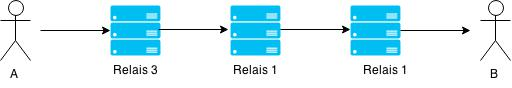
\includegraphics[scale=0.8]{project.jpg}
		\caption{Transfert d'un message de A vers B en passant par 3 relais}
		\label{project}
	\end{figure}
	
	\subsection{WebSocket}
	\paragraph*{}
	La première partie de notre PJI fut l'implémentation d'un réseau TOR à base de WebSocket entre des clients sous forme de navigateur web et un certains nombre de relais placé sur des serveurs web.
	\\\\
	\textit{\textbf{Qu'est-ce que les WebSocket ?}}
	\paragraph*{}
	WebSocket est une technologie très récente encore en cours de standardisation par le W3C et n'est disponible que sur les navigateurs les plus récents.
	Selon la définition officielle, je cite : \\
	\begin{quotation}
	WebSocket est une technologie évoluée qui permet d'ouvrir un canal de communication interactif entre un navigateur (côté client) et un serveur. \\Avec cette API vous pouvez envoyer des messages à un serveur et recevoir ses réponses de manière événementielle sans avoir à aller consulter le serveur pour obtenir une réponse.
	\end{quotation}
	\paragraph*{}
	Cette technologie correspond donc parfaitement à notre problématique.
	\paragraph*{}
	A partir de la, il  nous a fallu choisir quelle librairie de websocket utiliser car il en existe une infinité qui fleurisse chaque jour sur le net. Mais parmi toutes ces librairies, deux ont retenu notre attention tout particulièrement :
	\\
	\begin{itemize}
		\item[•] WebSocket API 
		\item[•] Socket.IO
	\end{itemize}		
	\paragraph*{}
	\subsubsection{WebSocket API}
	\paragraph*{}
	WebSocket API est tout simplement la librairie officielle supportée et en cours de standardisation par le W3C.
	Il nous était donc tout naturel de choisir cette librairie, ce que nous avons fait dans un premier temps.
	\paragraph*{}
	\textit{\textbf{Implémentation côté client}} 
	\paragraph*{}
	La première instruction est l'instanciation d'un objet WebSocket afin d'ouvrir une connexion avec le serveur.
	\paragraph*{}
	\begin{lstlisting}
var websocket = new WebSocket("ws://127.0.0.1:9000");
	\end{lstlisting}
	\paragraph*{}
	Remarquez le protocole utilisé qui n'est pas \emph{http} mais \emph{ws}. 
	On ne remarque pas vraiment la différence entre ces deux protocoles côté client mais c'est côté serveur que tout va changer.
	En effet, voila à quoi ressemble l'entête d'un paquet envoyé du protocole \emph{ws} :
	\paragraph*{}
	\begin{lstlisting}
GET /chat HTTP/1.1
Host: server.example.com
Upgrade: websocket
Connection: Upgrade
Sec-WebSocket-Key: x3JJHMbDL1EzLkh9GBhXDw==
Sec-WebSocket-Protocol: chat, superchat
Sec-WebSocket-Version: 13
Origin: http://example.com
	\end{lstlisting}
	\paragraph*{}
	On appelle ce paquet en anglais un \emph{WebSocket handshake request}, ce qui se traduit en français par une requête \emph{poignée de main}, c'est à dire que le client tend la main au serveur (fais une demande de connexion) et attend un retour positif du serveur afin d'établir une connexion correcte.
	\paragraph*{}
	Voici le paquet attendu par le client du serveur :
	\begin{lstlisting}
HTTP/1.1 101 Switching Protocols
Upgrade: websocket
Connection: Upgrade
Sec-WebSocket-Accept: HSmrc0sMlYUkAGmm5OPpG2HaGWk=
Sec-WebSocket-Protocol: chat
	\end{lstlisting}	
	\paragraph*{}
	Une fois ce paquet du serveur réceptionné, le client est connecté de manière persistante avec le serveur.
	\paragraph*{}
	La suite du code est l'implémentation d'une série d'événements.
	\paragraph*{}
	Ouverture de connexion
	\begin{lstlisting}
	websocket.onopen = function(ev) { // connection is open 
		$('#message_box').append("<div class=\"system_msg\">Connected!</div>"); //notify user
	}
	\end{lstlisting}	
	\paragraph*{}
	Fermeture de connexion
	\begin{lstlisting}
	websocket.onclose 	= function(ev){
		$('#message_box').append("<div class=\"system_msg\">Connection Closed</div>");
	}; 
	\end{lstlisting}	
	\paragraph*{}
	Erreur de connexion
	\begin{lstlisting}
	websocket.onerror	= function(ev){ 
		$('#message_box').append("<div class=\"system_error\">Error Occurred - "+ev.data+"</div>");
	}; 
	\end{lstlisting}	
	\paragraph*{}
	Réception d'un message du serveur
	\begin{lstlisting}
	websocket.onmessage = function(ev) {
		var msg = JSON.parse(ev.data); //PHP sends Json data
		var type = msg.type; //message type
		var umsg = msg.message; //message text
		var uname = msg.name; //user name
		var ucolor = msg.color; //color

		if(type == 'usermsg') 
		{
			$('#message_box').append("<div><span class=\"user_name\" style=\"color:#"+ucolor+"\">"+uname+"</span> : <span class=\"user_message\">"+umsg+"</span></div>");
		}
		if(type == 'system')
		{
			$('#message_box').append("<div class=\"system_msg\">"+umsg+"</div>");
		}
		
		$('#message').val(''); //reset text
		$("#message_box").scrollTop($("#message_box")[0].scrollHeight);
	};
	\end{lstlisting}	
	\paragraph*{}
	Puis dernier bout de code, l'envoi d'un message par le biais d'un simple tchat
	\begin{lstlisting}
	$('#send-btn').click(function(){ //use clicks message send button	
		var mymessage = $('#message').val(); //get message text
		var myname = $('#name').val(); //get user name
		
		if(myname == ""){ //empty name?
			alert("Enter your Name please!");
			return;
		}
		if(mymessage == ""){ //emtpy message?
			alert("Enter Some message Please!");
			return;
		}
		
		//prepare json data
		var msg = {
			message: mymessage,
			name: myname,
			color : '<?php echo $colours[$user_colour]; ?>',
			nodes : ["192.168.33.10:9002", "192.168.33.10:9001"] // node path to the client
		};
		//convert and send data to server
		websocket.send(JSON.stringify(msg));
	});
	\end{lstlisting}	
	\paragraph*{}
	\textit{\textbf{Implémentation côté client}} 
	\paragraph*{}
	La librairie officielle des WebSocket n'est à ce jour implémentée que pour le côté client. 
	\paragraph*{}
	Nous avons choisi PHP pour développé le serveur mais PHP ne propose aucune librairie officielle pour communiquer correctement avec le protocole \emph{ws}. 
	\paragraph*{}
	Nous avons donc pris l'initiative de développer nous même une implémentation du protocole \emph{ws} en PHP.
	\paragraph*{}
	Nous détaillerons pas ici le code de cette implémentation car il est long et complexe et il nous permet pas de nous concentrer sur le cœur de notre PJI.
	\paragraph*{}
	Au final, nous avons pris la décision de passer sous NodeJS et d'utiliser la librairie \emph{Socket.IO} qui est bien plus simple à utiliser et nous permet de nous concentrer sur le cœur du projet initial.
	\subsubsection{Socket.IO}
	\paragraph*{}
	Socket.IO est une librairie pour le serveur JavaScript NodeJS. \\
	L'avantage de cette librairie est qu'en plus de sa simplicité déconcertante à utiliser, le code est le même que ce soit côté client ou côté serveur puisque le langage utilisé est le même (JavaScript). 
	\paragraph*{}
	\textit{\textbf{Implémentation côté client}} 
	\paragraph*{}
	Ouverture de connexion avec le serveur
	\begin{lstlisting}
var socket = io.connect('http://127.0.0.1:9000');
	\end{lstlisting}
	\paragraph*{}
	Gestion des événements 
	\begin{lstlisting}
	socket.on('connect', function() {
		...
	});

	socket.on('disconnect', function() {
		...
	});

	socket.on('error', function() {
		...
	});

	socket.on('msg', function(msg) {
		...
	});
	\end{lstlisting}	
	\paragraph*{}
	Envoi d'un message 
	\begin{lstlisting}
	$('#send-btn').click(function() { //use clicks message send button	
		...
	    	//prepare json data
			var msg = {
				message: encryptedMsg,
				name: myname,
				color : user_colour,
				nodes : nodes_list // node path to the client
			};

			//send data to server
			socket.emit('msg', msg);
		...
	});
	\end{lstlisting}		 
	\paragraph*{}
	\textit{\textbf{Implémentation côté serveur}} 
	\paragraph*{}
	Création d'un serveur web 
	\begin{lstlisting}
var http = require('http');

httpServer = http.createServer(function(req, res) {
	res.end('Hello World');
});

httpServer.listen(port);
	\end{lstlisting}			
	\paragraph*{}
	Création d'une socket serveur écoutant sur le serveur web 
	\begin{lstlisting}
var io = require('socket.io').listen(httpServer);
	\end{lstlisting}	
	\paragraph*{}
	Réception des connexions clientes
	\begin{lstlisting}
io.sockets.on('connection', function(socket) {
	console.log('new user');
	...
});
	\end{lstlisting}
	\paragraph*{}
	Réception des messages
	\begin{lstlisting}
	socket.on('msg', function(msg) {
		msg.type = 'usermsg';
		
		// Envoi le message a tous les clients connectes
		io.sockets.emit('msg', msg);

		// Envoi le message au relais suivant
		if(msg.nodes.length > 0) {
			...	
		}
	});
	\end{lstlisting}		
	
	
	\subsection{Web Cryptography}
	\paragraph*{}
	Afin de bien crypter les messages envoyés et d'utiliser une technologies assez fiable et récente, nous avons privilégié la Web Cryptography API. En effet, elle est compatible sur presque tous les navigateurs (inclus de base). En revanche, il nous a fallu trouver un bon algorithme de chiffrement.\\
	Dans un premier temps, nous avons utilisé le chiffrement AES-CBC afin de tester et découvrir Webcrypto API et réaliser un premier jet de ce que nous voulions faire. Une fois le messages encrypté 4 fois. Voici un exemple du cryptage :
	\newpage	
	\begin{figure}[h] %%%%% h = here, t = top, b = bottom
		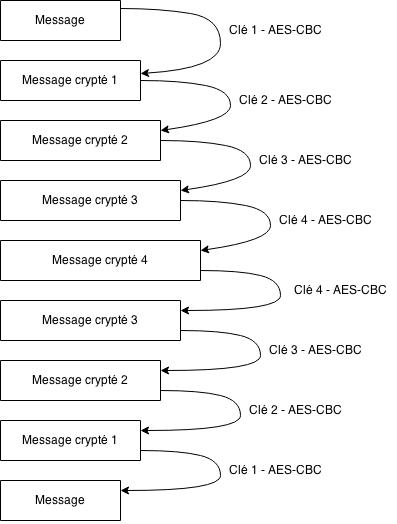
\includegraphics[scale=0.70]{AES.jpg}
		\caption{Cryptage d'un message 4 fois de suite en AES-CBC}
		\label{AES}
	\end{figure}
	\paragraph*{}
	Pour la solution optimale, il est plus préférable d'utiliser un système de clés publiques et de clés privées. Avec l'algorithme RSA-OAEP, cela est possible. Chaque clé générée (l'objet KeyPromise) contient une clé publique et une clé privée. De ce fait, cette solution est plus attendu car elle ressemble très fortement à l'architecture du réseau TOR. Bien entendu, le client doit connaître le chemin afin qu'il puisse créer son message crypté avec les clés publiques des relais correspondants.
	\paragraph*{}
	Ce qu'il faut comprendre en utilisant WebCrypto API, c'est le fait que pour générer une clé, encrypter ou décrypter, nous jouons avec des \textit{Promises}. En JavaScript, des \textit{Promises} ou "promesses" en français, sont utilisées pour réaliser des actions asynchrones. En effet, elles représentent des intermédiaires vers des valeurs qui ne sont nécessairement connues lors de leurs créations. Cela permet de gérer des actions asynchrones et de leur associer des gestionnaires d'erreurs. 
	\paragraph*{}
	La principale difficulté qui réside dans le fait d'utiliser des \textit{Promises} est de bien gérer les erreurs mais savoir exactement où le code à échouer. Le fait d'encrypter un message avec une clé publique puis d'encrypter le résultat avec une autre clé publique nécessite obligatoirement une imbrication du code.
	Voici un exemple :
	\begin{lstlisting}
window.crypto.subtle.generateKey({name: "aes-cbc", length: 128}, true, ["encrypt", "decrypt"]).then(function (key) {
  var data = asciiToUint8Array("ceci est un test");
  console.log("Data:");
  console.log("value: ceci est un test")
  console.log(data);
  var algorithm = key.algorithm;
  algorithm.iv = window.crypto.getRandomValues(new Uint8Array(16));

  window.crypto.subtle.encrypt(algorithm, key, data).then(function (ct) {
    console.log("AES-CBC encrypt 1:");
    console.log(new Uint8Array(ct));

    window.crypto.subtle.decrypt(algorithm, key, ct).then(function (pt) {
      console.log("AES-CBC decrypt 1:");
      console.log(new Uint8Array(pt));
      console.log(uint8ArrayToAscii(new Uint8Array(pt)));
    }, handle_error);
  }, handle_error);
}, handle_error);
	\end{lstlisting}
	\paragraph*{}
	Une autre difficulté réside dans le fait de trouver un bon algorithme qui respecte ce que l'on souhaite faire. Par exemple, pour découvrir WebCrypto API, nous avions testé avec la cryptographie AES-CBC comme dans l'exemple précédent.
	Dans ce cas, on constate que l'on a bien une clé qui est générée. En revanche, elle ne respecte par ce que l'architecture TOR exige. La clé n'est pas publique ni privée mais permet juste d'encrypter un message et de le décrypter. Nous avons regardé les différents cryptages disponibles et compatibles et nous avons trouvé RSA-OAEP. Ce dernier gère les clés publiques et privées et permet d'encrypter et de décrypter. D'autres cryptographies RSA possèdent juste les fonctions de signature et de vérification de la signature. Également, la cryptographie RSAES-PKCS1-v1\_5	 aurait pu être exploitée mais cette dernière n'est plus disponible dans les navigateurs. C'est donc pour cela que nous avons choisi RSA-OAEP.\\
	Voici un exemple basique avec RSA-OAEP :
	\begin{lstlisting}
window.crypto.subtle.generateKey({name: "RSA-OAEP", modulusLength: 2048, publicExponent: new Uint8Array([0x01, 0x00, 0x01]), hash: {name: "SHA-256"}}, true, ["encrypt", "decrypt"]).then(function (key) {
  var data = asciiToUint8Array("ceci est un test");
  console.log("Data:");
  console.log(uint8ArrayToAscii(data));
  console.log("Public Key");
  console.log(key.publicKey);
  console.log("Private Key");
  console.log(key.privateKey);

  window.crypto.subtle.encrypt({name: "RSA-OAEP"}, key.publicKey, data).then(function (encrypted) {
    console.log(uint8ArrayToAscii(new Uint8Array(encrypted)));

    window.crypto.subtle.decrypt({name: "RSA-OAEP"}, key.privateKey, encrypted).then(function (decrypted) {
      console.log(uint8ArrayToAscii(new Uint8Array(decrypted)));
    }, handle_error);
  }, handle_error);
}, handle_error);
	\end{lstlisting}
	\paragraph*{}
	Également, nous avons pu regarder quels sont les algorithmes supportés par la plupart des navigateurs. Nous en avons donc dressé le tableau suivant : 
	\begin{center}
	\begin{tabular}[h]{|*{2}{c|}}
  		\hline
  		Algorithme & Supporté\\
  		\hline
  		RSASSA-PKCS1-v1\_5 & Oui\\
  		\hline
  		RSAES-PKCS1-v1\_5 & Non\\
  		\hline
  		RSA-PSS & Oui\\
  		\hline
  		RSA-OAEP & Oui\\
  		\hline
  		AES-CTR & Oui\\
  		\hline
  		AES-CBC & Oui\\
  		\hline
  		AES-CMAC & Non\\
  		\hline
  		AES-GCM & Oui\\
  		\hline
  		AES-CFB & Oui\\
  		\hline
  		AES-KW & Oui\\
  		\hline
  		SHA-1 & Oui\\
  		\hline
  		SHA-256 & Oui\\
  		\hline
  		SHA-384 & Oui\\
  		\hline
  		SHA-512 & Oui\\
  		\hline
	\end{tabular}
	\end{center}
	Les algorithmes SHA sont des \textit{digest}. Cela sert principalement à créer des table de hachage crypter un message ou une clé par exemple. Dans le code précédent, on peut remarquer que la fonction de hachage mise en place est bien le SHA-256.
	\paragraph*{}
	Une fois que nous avions trouvé l'algorithme et trouver son fonctionnement, nous avons du mettre en place une maquette. Voici donc une image représentative de ce que l'on a testé :
	\begin{figure}[h] %%%%% h = here, t = top, b = bottom
		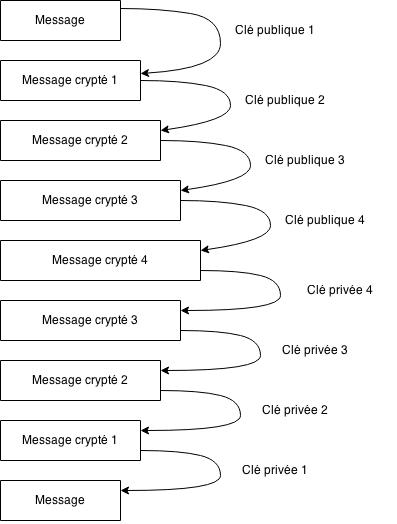
\includegraphics[scale=0.70]{RSA.jpg}
		\caption{Cryptage d'un message 4 fois de suite en RSA-OAEP}
		\label{RSA}
	\end{figure}
	\\
	Dans cet exemple, il faut crypter obligatoirement avec la clé publique et décrypter avec la clé privée correspondante. En effet, les clés publiques sont accessibles à tout le monde alors que les clés privées sont uniquement restreintes au point relais correspondant.

	\subsection{Architecture de l'application}
	\paragraph*{}
	L'application se compose en 3 parties :\\
	\begin{itemize}
		\item[•]WebCrypto
		\item[•]Websocket en PHP
		\item[•]Websocket en NodeJS
	\end{itemize}
	Dans chacune des parties, un README est fourni précisant comment tester la partie concernée. Ces derniers sont écrits en markdown.
	\paragraph*{}
	La partie Webcrypto comprends une page html ainsi que plusieurs fichiers JavaScript dans le dossier js/. Dans ce dernier dossier, on y retrouve les tests de base en AES-CBC puis en RSA-OAEP.\\
	Voici les fichiers dans le dossier Webcrypto part : \\
	\begin{itemize}
		\item[•]index.html
		\item[•]js/
		\begin{itemize}
			\item[•]jquery-1.11.2.min.js
			\item[•]short-cbc.js
			\item[•]short-rsa.js
			\item[•]test-cbc.js
			\item[•]test-rsa.js
		\end{itemize}
	\end{itemize}
	Par défaut, la page index.html utilise le fichier test-rsa.js.
	\paragraph*{}
	Pour la partie utilisant NodeJS, nous avons plusieurs dossiers et fichiers
	Voici la composition :\\
	\begin{itemize}
		\item[•]lib/ \hspace{72px} dossier contenant les librairies
		\item[•]js/ \hspace{80px} dossier contenant le code JavaScript pour le client et Socket.io
		\item[•]node\_modules/ \hspace{10px} dossier contenant les modules pour NodeJS
		\item[•]css/
		\item[•]client1.html
		\item[•]client2.html
		\item[•]server.js
		\item[•]package.json
	\end{itemize}
	\paragraph*{}
	Pour la partie PHP, il y a juste 2 fichiers : \\
	\begin{itemize}
		\item[•]index.html
		\item[•]server.php
	\end{itemize}
	Comme leurs noms l'indique, la page index.html correspond au client et server.php au server.

\newpage	
\section{Mode d'emploi}
	\subsection{Installer et configurer les relais}
	\paragraph*{}
	Dans un premier temps, nous supposons que NodeJS est installé et fonctionnel en ligne de commande.
	\paragraph*{}
	La première chose à faire est d'installer toutes les dépendances au bon fonctionnement du relais, c'est à dire tous les modules NodeJS dont le programme à besoin pour fonctionner.
	\paragraph*{}
	Grâce à un fichier \emph{package.json} qui décrit toutes les dépendances à installer, il suffit de taper la commande : (dans le même dossier au se trouve le fichier \emph{package.json})
	
	\begin{lstlisting}
npm install
	\end{lstlisting}
	
	\paragraph*{}
	Un dossier \emph{node\_modules} sera créé contenant les dépendances.
	
	\paragraph*{}
	Nous pouvons maintenant démarrer autant de relais que nous le souhaitons via la commande :
	
	\begin{lstlisting}
node server.js [<num_port>]
	\end{lstlisting}	
	
	\paragraph*{}
	Évidemment, nous mettons un numéro de port différent pour chaque relais. Dans le cas où aucun numéro n'est précisé, il s'agit du port 9000.
	
	\subsection{Installer et configurer les clients}
	\paragraph*{}
	Les clients sont sous forme de simple fichiers html. (ex: client1.html)
	
	\paragraph*{}
	Cependant, nous devons quand même regarder le code pour les configurer. \\
	En effet, il faut définir l'adresse des relais à parcourir pour envoyer un message.
	
	\paragraph*{}
	Ouvrons le fichier \emph{client1.html} et regardons le code.
	
	\paragraph*{}
	\begin{lstlisting}
var node_addr = 'http://127.0.0.1:9000';
	\end{lstlisting}	
	
	\paragraph*{}
	Cette ligne décrit le relais qui aura une connexion permanente avec le client. \\
	C'est également le relais qui recevra en premier tous les messages du client.
	
	\paragraph*{}
	\begin{lstlisting}
var nodes_list = ["127.0.0.1:9001", "127.0.0.1:9002"];
	\end{lstlisting}	
	
	\paragraph*{}
	Cette ligne décrit la liste des relais suivant à parcourir. \\
	Les clients qui recevront les messages doivent être connectés au dernier relais de la liste.	

	\subsection{Lancer l'application}
	\paragraph*{}
	Prenons pour exemple cette figure :
	
	\begin{figure}[h] %%%%% h = here, t = top, b = bottom
		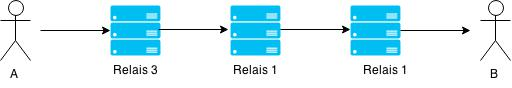
\includegraphics[scale=0.8]{project.jpg}
		\caption{Transfert d'un message de A vers B en passant par 3 relais}
		\label{project}
	\end{figure}
	
	\paragraph*{}
	Nous sommes un client A et nous voulons envoyer un message au client B en passant par 3 relais d'adresse :
	
	\paragraph*{}
	\begin{itemize}
		\item[•]Relais 3 : 127.0.0.1:9000
		\item[•]Relais 2 : 127.0.0.1:9001
		\item[•]Relais 1 : 127.0.0.1:9002
	\end{itemize}
	
	\paragraph*{}
	En revanche le client B n'envoie pas de message au client A.
	
	\paragraph*{}
	Tout d'abord nous configurons les relais ainsi que les clients comme décrit ci-dessus. \\
	Les relais se lancent avec les commandes :
	
	\paragraph*{}
	\begin{lstlisting}
node server.js 9000
node server.js 9001
node server.js 9002
	\end{lstlisting}
	
	\paragraph*{}
	Le client A se configure ainsi :
	
	\paragraph*{}
	\begin{lstlisting}
	var node_addr = 'http://127.0.0.1:9000';
	var nodes_list = ["127.0.0.1:9001", "127.0.0.1:9002"];
	\end{lstlisting}	
	
	\paragraph*{}
	Le client B se configure ainsi :
	
	\paragraph*{}
	\begin{lstlisting}
	var node_addr = 'http://127.0.0.1:9002';
	var nodes_list = [];
	\end{lstlisting}
	
	\paragraph*{}
	Maintenant, nous ouvrons le tchat et arrivons sur cette page :
	
	\begin{figure}[h] %%%%% h = here, t = top, b = bottom
		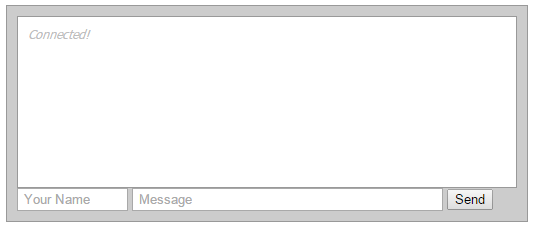
\includegraphics[scale=0.8]{chat_connected.png}
		\caption{Le client A est bien connecté au relais 3}
		\label{project}
	\end{figure}	
	
	\paragraph*{}
	Un message système nous informe que la connexion s'est effectué correctement au premier relais. \\
	Nous pouvons alors envoyer des messages au client B.
	
	\begin{figure}[h] %%%%% h = here, t = top, b = bottom
		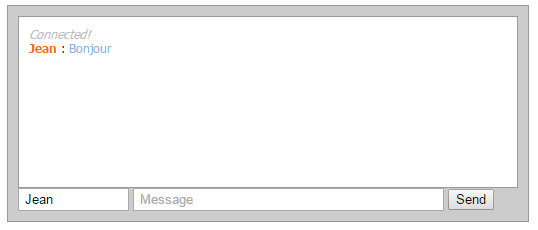
\includegraphics[scale=0.8]{chat_message.png}
		\caption{Le relais nous renvoie le message envoyé}
		\label{project}
	\end{figure}	
	
	
\newpage	
\section{Tests}
	\subsection{WebSocket}
	\paragraph*{}
	Ici, nous nous intéresserons à la partie NodeJS seulement car c'est la partie finale qui a été choisi pour ce PJI.	
	
	\paragraph*{}
	Le premier test à effectuer avec NodeJS est si le serveur est bien démarré ou non. 
	
	\begin{figure}[h] %%%%% h = here, t = top, b = bottom
		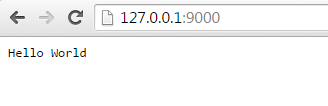
\includegraphics[scale=0.8]{started_server.png}
		\caption{Le serveur est démarré correctement}
		\label{project}
	\end{figure}
	
	\paragraph*{}
	Sur cette figure, nous pouvons visualiser un \emph{Hello World} lorsque nous tapons l'adresse du relais dans le navigateur. Le serveur est donc bien démarré.
	
	\paragraph*{}
	Le code se rapportant au démarrage du serveur est le suivant :
	
	\paragraph*{}
	\begin{lstlisting}
httpServer = http.createServer(function(req, res) {
	res.end('Hello World');
});

httpServer.listen(port);
	\end{lstlisting}	
	
	\paragraph*{}
	Nous voulons tester que le relais reçoit bien la connexion d'un client \\
	Pour cela, il faut d'abord créer une instance d'une socket serveur comme ceci :
	
	\paragraph*{}
	\begin{lstlisting}
var io = require('socket.io').listen(httpServer);
	\end{lstlisting}
	
	\paragraph*{}
	Cette ligne importe un nouveau module NodeJS, il faut donc que ce module soit bien installé au projet. \\
	Si aucune erreur apparaît lors du démarrage du relais alors le module est installé correctement.
	
	\paragraph*{}
	Voici le code qui écoute la connexion des socket clientes :

	\paragraph*{}
	\begin{lstlisting}
io.sockets.on('connection', function(socket) {
	console.log('new user');
	
	...
});
	\end{lstlisting}
	
	\paragraph*{}
	A chaque connexion d'un client au relais, la console affiche donc \emph{new user}.
	
	\paragraph*{}
	Nous voulons tester que le relais reçoit bien un message client et le renvoi correctement à tous les clients connectés. 
	
	\paragraph*{}
	\begin{lstlisting}
	socket.on('msg', function(msg) {
		...
		io.sockets.emit('msg', msg);

		...
	});
	\end{lstlisting}	
	
	\paragraph*{}
	Si le code fonctionne, tous les clients connectés reçoivent le message.
		
	\paragraph*{}
	Le dernier test est de vérifier que le relais traite bien le message qu'il a reçu et renvoi le message au relais suivant le chemin donné dans le message.
	
	\paragraph*{}
	\begin{lstlisting}
		if(msg.nodes.length > 0) {
			var next_node = 'http://' + msg.nodes[0];
			msg.nodes = msg.nodes.slice(1);

			if(!io_client_connected) {
				io_client = require("socket.io-client")(next_node);
			} else {
				io_client.emit('msg', msg);			
			}

			io_client.on('connect', function() {
				io_client_connected = true;
				io_client.emit('msg', msg);
			});

			io_client.on('disconnect', function() {
				io_client_connected = false;
			});	
		}
	\end{lstlisting}
	
	\paragraph*{}
	Ici, il faut avoir installé le module \emph{socket.io-client} car pour se connecter au prochain relais de la liste, le relais devient client.
		 
	
	\subsection{Cryptographie}
	\paragraph*{}
	Pour la cryptographie avec WebCrypto API, il fallait tester des cas de base. Tout d'abord pour découvrir le fonctionnement, nous avons pris l'algorithme AES-CBC. Puis nous avons généré une clé et encrypté un message de test. Une fois ce message encrypté, nous avons affiché le résultat sous la forme d'une chaîne de caractères. Ensuite, pour vérifier que l'on puisse bien décrypter cela, nous l'avons décrypter avec la clé et vérifié que le message décrypté correspondait bien à celui de départ.\\
	Voici le code qui a permis de réaliser cela :
	\begin{lstlisting}
window.crypto.subtle.generateKey({name: "aes-cbc", length: 128}, true, ["encrypt", "decrypt"]).then(function (key) {
  var data = asciiToUint8Array("ceci est un test");
  console.log("Data:");
  console.log("value: ceci est un test")
  console.log(data);
  var algorithm = key.algorithm;
  algorithm.iv = window.crypto.getRandomValues(new Uint8Array(16));

  window.crypto.subtle.encrypt(algorithm, key, data).then(function (ct) {
    console.log("AES-CBC encrypt 1:");
    console.log(new Uint8Array(ct));

    window.crypto.subtle.decrypt(algorithm, key, ct).then(function (pt) {
      console.log("AES-CBC decrypt 1:");
      console.log(new Uint8Array(pt));
      console.log(uint8ArrayToAscii(new Uint8Array(pt)));
    }, handle_error);
  }, handle_error);
}, handle_error);
	\end{lstlisting}
	Une fois ceci réalisé, nous nous sommes posés la question de ce qu'il en est si nous cryptons 4 fois de suite un message. Pour cela, il nous a fallu adapter notre code de manière basique et de tester ce que cela donnait.\\
	Voici l'enchaînement du code : 
	\begin{lstlisting}
function startCrypto(input_content){
  window.crypto.subtle.generateKey({name: "aes-cbc", length: 128}, true, ["encrypt", "decrypt"]).then(function (key1) {
    var data = asciiToUint8Array(input_content);
    var algorithm = key1.algorithm;
    algorithm.iv = window.crypto.getRandomValues(new Uint8Array(16));

    window.crypto.subtle.generateKey({name: "aes-cbc", length: 128}, true, ["encrypt", "decrypt"]).then(function (key2) {
      var algorithm = key2.algorithm;
      algorithm.iv = window.crypto.getRandomValues(new Uint8Array(16));

      window.crypto.subtle.generateKey({name: "aes-cbc", length: 128}, true, ["encrypt", "decrypt"]).then(function (key3) {
        var algorithm = key3.algorithm;
        algorithm.iv = window.crypto.getRandomValues(new Uint8Array(16));

        window.crypto.subtle.generateKey({name: "aes-cbc", length: 128}, true, ["encrypt", "decrypt"]).then(function (key4) {
          var algorithm = key4.algorithm;
          algorithm.iv = window.crypto.getRandomValues(new Uint8Array(16));

          window.crypto.subtle.encrypt(algorithm, key1, data).then(function (ct1) {
            console.log("AES-CBC encrypt 1:");
            console.log(uint8ArrayToAscii(new Uint8Array(ct1)));

            window.crypto.subtle.encrypt(algorithm, key2, new Uint8Array(ct1)).then(function (ct2) {
              console.log("AES-CBC encrypt 2:");
              console.log(uint8ArrayToAscii(new Uint8Array(ct2)));

              window.crypto.subtle.encrypt(algorithm, key3, new Uint8Array(ct2)).then(function (ct3) {
                console.log("AES-CBC encrypt 3:");
                console.log(uint8ArrayToAscii(new Uint8Array(ct3)));

                window.crypto.subtle.encrypt(algorithm, key4, new Uint8Array(ct3)).then(function (ct4) {
                  console.log("AES-CBC encrypt 4:");
                  console.log(uint8ArrayToAscii(new Uint8Array(ct4)));

                  window.crypto.subtle.decrypt(algorithm, key4, ct4).then(function (pt4) {
                    console.log("AES-CBC decrypt 4:");
                    console.log(uint8ArrayToAscii(new Uint8Array(pt4)));

                    window.crypto.subtle.decrypt(algorithm, key3, pt4).then(function (pt3) {
                      console.log("AES-CBC decrypt 3:");
                      console.log(uint8ArrayToAscii(new Uint8Array(pt3)));

                      window.crypto.subtle.decrypt(algorithm, key2, pt3).then(function (pt2) {
                        console.log("AES-CBC decrypt 2:");
                        console.log(uint8ArrayToAscii(new Uint8Array(pt2)));

                        window.crypto.subtle.decrypt(algorithm, key1, pt2).then(function (pt) {
                          console.log("AES-CBC decrypt 1:");
                          console.log(uint8ArrayToAscii(new Uint8Array(pt)));
                        }, handle_error);
                      }, handle_error);
                    }, handle_error);
                  }, handle_error);
                }, handle_error);
              }, handle_error);
            }, handle_error);
          }, handle_error);
        }, handle_error);
      }, handle_error);
    }, handle_error);
  }, handle_error);
}
	\end{lstlisting} 
	Comme on peut le constater le code devient de plus en plus en illisible si on l'imbrique. Cependant, étant juste le test de découverte, cela avait peut d'importance mais il s'agissait juste de la manière de procéder qui nous intéressait. De ce fait, nous avons appliqué ceci avec la bon cryptage qui est RSA-OAEP. pour le cas d'un seul encryptage, il s'agit a peu de chose près le même cas que AES-CBC. En revanche, pour un encryptage multiple, cela dépend de la taille des données. En effet, nous avons voulu faire varier le \textit{modulusLength}. Cela nous a permis d'avoir un message crypté plus ou moins grand.\\ L'exemple suivant nous a permis de réaliser cela : 
	\begin{lstlisting}
function generateKeys(){
  window.crypto.subtle.generateKey({name: "RSA-OAEP", modulusLength: 512, publicExponent: new Uint8Array([0x01, 0x00, 0x01]), hash: {name: "SHA-1"}}, true, ["encrypt", "decrypt"]).then(function (key) {
    keyGenerate1 = key;
    console.log(keyGenerate1);
    window.crypto.subtle.generateKey({name: "RSA-OAEP", modulusLength: 1024, publicExponent: new Uint8Array([0x01, 0x00, 0x01]), hash: {name: "SHA-1"}}, true, ["encrypt", "decrypt"]).then(function (key2) {
      keyGenerate2 = key2;
      console.log(key2);
      window.crypto.subtle.generateKey({name: "RSA-OAEP", modulusLength: 2048, publicExponent: new Uint8Array([0x01, 0x00, 0x01]), hash: {name: "SHA-1"}}, true, ["encrypt", "decrypt"]).then(function (key3) {
        keyGenerate3 = key3;
        console.log(key3);
        window.crypto.subtle.generateKey({name: "RSA-OAEP", modulusLength: 4096, publicExponent: new Uint8Array([0x01, 0x00, 0x01]), hash: {name: "SHA-1"}}, true, ["encrypt", "decrypt"]).then(function (key4) {
          keyGenerate4 = key4;
          console.log(key4);
          alert("Cles generees");
        }, handle_error);
      }, handle_error);
    }, handle_error);
  }, handle_error);
}	
	\end{lstlisting}
	Une fois les clés générées, il ne nous restait plus qu'à les stocker afin de pouvoir les réutiliser par la suite. De plus, nous avons factoriser le code de l'encryptage et du décryptage afin d'éviter l'imbrication vu comme précédemment. 
		\begin{lstlisting}
function encryptData(key, data, jquerySelector){
  var temp;
  compteur += 1;
  window.crypto.subtle.encrypt({name: "RSA-OAEP"}, key.publicKey, data).then(function (ct1) {
    console.log("RSA-OAEP encrypt "+compteur+" :");
    temp = new Uint8Array(ct1);
    encryptedMsg = new Uint8Array(ct1);
    $( jquerySelector ).text($( jquerySelector ).text()+uint8ArrayToAscii(temp));
    console.log(uint8ArrayToAscii(temp));
  }, handle_error);
  return temp;
}

function decryptData(key, data, jquerySelector){
  window.crypto.subtle.decrypt({name: "RSA-OAEP"}, key.privateKey, data).then(function (pt) {
    console.log("RSA-OAEP decrypt "+compteur+" :");
    encryptedMsg = new Uint8Array(pt);
    $( jquerySelector ).text($( jquerySelector ).text()+uint8ArrayToAscii(encryptedMsg));
    console.log(uint8ArrayToAscii(encryptedMsg));
    compteur -= 1;
    return pt;
  }, handle_error);
}	
	\end{lstlisting}
	L'utilisation de \textit{console.log()} nous a été très utile afin de debugger notre code mais aussi servir de trace pour voir l'utilisation de ce dernier. Une fois ceci fait, l'enchaînement des cryptages et décryptages se fait séquentiellement.\\
	Un exemple est disponible dans la partie ./Webcrypto part/ en affichant la page index.html.

\newpage	
\begin{center}
\section*{Conclusion}
\end{center}
\paragraph*{}
Ce projet est très formateur autant dans l'aspect que dans la complexité des technologies. Nous avons passé beaucoup de temps sur NodeJS mais aussi sur Webcrypto API afin de bien comprendre et bien vérifier nos tests afin que tout soit correct. Avec ce projet, nous avons reçu beaucoup de connaissance sur la cryptographie mais aussi sur l'utilisation et la configuration de NodeJS.
\paragraph*{}
Cependant, étant des technologies encore très récentes et en cours de développement, nous avons pu commencer à utiliser ces technologies qui seront développées et utilisées de plus en plus  dans un futur proche. Or, tout n'est pas spécialement développé sur ces technologies.
\paragraph*{}
Pour terminer complètement ce projet l'idéal serait développer un module ou une librairie afin de faire communication entre Webcrypto API et la cryptographie inclue dans NodeJS. Cela consiste en la suite logique et complète du projet. 

\end{document}